\section{Erstellung}
Hierfür müssen zunächst einmal Testfälle in eine Ontologie umgewandelt werden. Um ein ausreichend großes Beispiel zu bieten, wird hierfür der BAYOOSOFT Access Manager verwendet, für den bereits im Rahmen des dieser Arbeit zugehörigen Praxisprojekts ein Konzept zur Testautomatisierung entworfen wurde. Um die folgenden Ontologien zu entwerfen wurde Protégé verwendet und das Ergebnis anschließend in WebVOWL visualisiert. \newline
Eine einfache Ontologie für die Testfälle von der Berechtigungsvergabe könnte so aussehen:\\

\begin{center}
    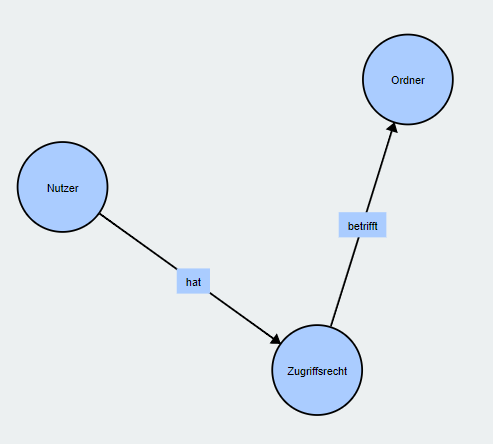
\includegraphics[width=1\textwidth]{Thesis/Images/OntologySmall.png}    
\end{center}
%\piccaption{Vereinfachte Ontologiedarstellung für die Vergabe von Zugriffsrechten im Access Manager}

In dieser Ontologie werden stark vereinfacht die Funktion des Vergebens von Zugriffsrechten auf Ordnern zusammengefasst. Verwendet man die Ontologie nun auf spezielle Ausprägungen mit den für das System bekannten Daten (Zugriffsrechte umfassen Lese- und Schreibrechte) und Testdaten wie verschiedene Nutzer oder Ordner, ergeben sich verschiedene Testfälle, die die hier dargestellte Funktionalität abdecken. So hat z.B. Nutzer A Schreibrechte auf Ordner Y, aber hat keinen Zugriff auf Ordner Z. \\

Um nun weitere Aspekte des Produkts und seiner Umgebung zu berücksichtigen, wird die Ontologie um einige Knoten und Kanten erweitert. \\

\begin{center}
    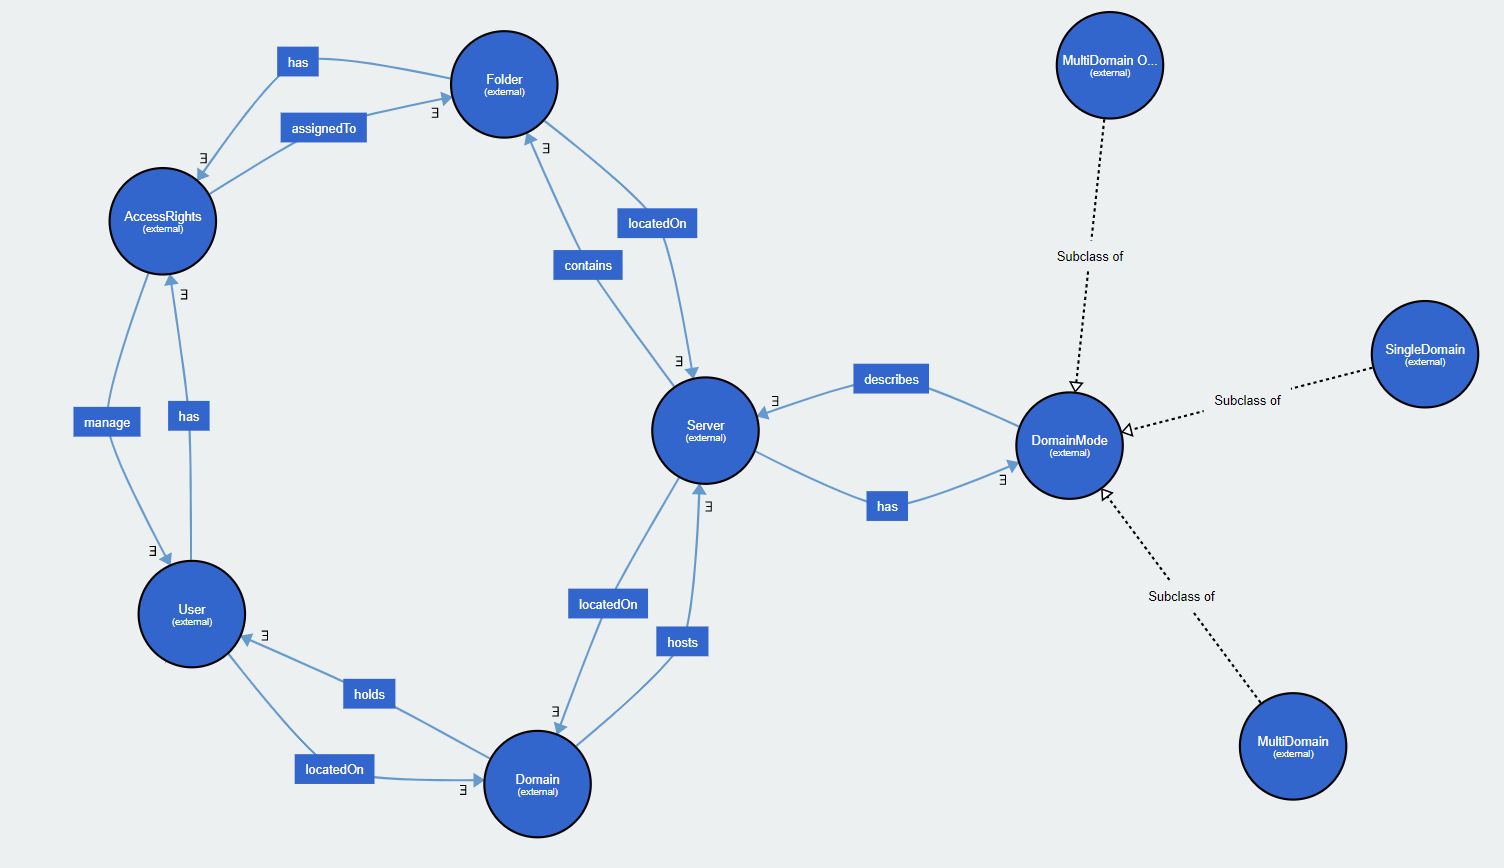
\includegraphics[width=1\textwidth]{Thesis/Images/OntologyBig.png}
\end{center}
%\piccaption{Umfassende Ontologiedarstellung für die Vergabe von Zugriffsrechten im Access Manager}

Es werden nun zusätzlich noch Domänen der Nutzer und der Ordner bzw. Server berücksichtigt sowie der Domainmode, was einige Einschränkungen mit sich bringt, wenn es daran geht die Ontologie mit bekannten Daten zu verwenden. So kann auf einem Ordner, der sich auf einem Server mit Singledomain Domainmode befindet, kein User aus einer anderen Domäne berechtigt sein. Dadurch können jetzt wesentlich mehr Testfälle dargestellt werden. 
